%% 2-line examples (2x3)
\begin{figure}
\begin{center}
    \begin{subfigure}{0.4\linewidth}
        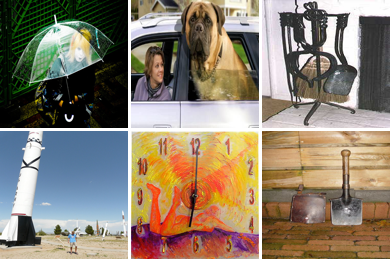
\includegraphics[width=\linewidth]{figures/imagenet_images/2x3grid_IN.png}
        \caption{{ImageNet} (pre-train)}
        \label{fig:imagenet}
    \end{subfigure}
    \quad
    \begin{subfigure}{0.4\linewidth}
        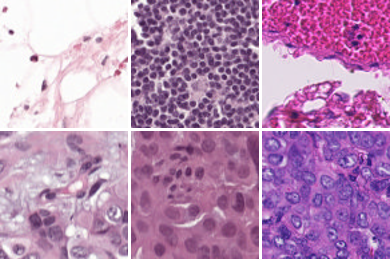
\includegraphics[width=\linewidth]{figures/camelyon_images/2x3grid_CM.png}
        \caption{\data{Camelyon17} (fine-tuning)}
        \label{fig:camelyon}
    \end{subfigure}

    \caption{\small \textbf{Example images of ImageNet and \data{Camelyon17}.} Large distribution shift occurs between pre-training ({ImageNet}) and fine-tuning (\data{Camelyon17}). ImageNet is a multiclass objective recognition task and \data{Camelyon17} is a binary classification task for reading whether the image contains tumor tissue. Instagram-3.6B examples are omitted since it is not publicly available.
    }
    \label{fig:imagenet_camelyon}
\end{center}
\end{figure}
